\chapter{Matchings and covers in bipartite graphs}

\section{Introduction}

Given a graph $G = (V,E)$, a \emph{matching} $M$ in $G$ is a set of pairwise non-adjacent edges; that is, no two edges share a common vertex. A \emph{maximum matching} is a matching that contains the largest possible number of edges.

A (\emph{vertex}) \emph{cover} $C$ in $G$ is a set of vertices such that for every edge $uv \in E$, either $u \in C$ or $v \in C$. A \emph{minimum cover} is a cover of the smallest possible size.

\subsection{Algorithm for bipartite graphs}

Maximum matching (and minumum cover) in bipartite graphs can be found in polynomial time using Max-Flow-Min-Cut algorithm (Ford Fulkerson).

\medskip
\noindent \textbf{Algorithm:}
\begin{enumerate}
\item Let $G$ be a bipartite graph with vertex bipartition $V(G) = A \cup B$.
\item Create a directed weighted graph $G^+$ with vertex set $V(G) \cup \{s, t\}$, i.e., add two vertices, source ($s$) and sink ($t$).
\item Edges of $G^+$ are edges $(s, a)$, $a \in A$, $(b, t)$, $b \in B$ and edges of the original graph directed from $A$ to $B$.
\item Put weight (capacity) $1$ to edges of type $(s, a)$ and $(b, t)$ and $\infty$ (a large integer, e.g., the number of vertices in $G$) to all other edges (edges between $A$ and $B$).
\item Compute (integer) max flow $f$ with source $s$ and sink $t$.
\item Maximum matching consist of edges $\{uv \in E(G) \mid f(u, v) = 1\}$.
\item Compute min cut $(S, T)$, such that $s \in S$ and $t \in T$.  Minimum cover of $G$ is set $C = \{v \in A \mid v \in T\} \cup \{v \in B \mid v \in S\}$
\end{enumerate}

\medskip
\noindent Why does this algortihm work?

\medskip
Let $f$ be the max flow (integral!) obtained in 5. Then the edge set in 6 is clearly a matching, since flow "coming" from the vertex $s$ to a vertex $a \in A$ has value 1 and, since it is integral, cannot "split" from $a$ towards two vertices in $B$ Also flow cannot "come" to a vertex $b \in B$ from two vertices in $A$, since it is integral and capacity of the edge $(b, t)$ is 1.

The reverse is also true, any matching $M$ produces a flow from $s$ to $t$ with value $|M|$. Therefore a max flow gives a max matching and a max matching gives a max flow.

What about min cut. The set $C$ from 7 is a cover, since every edge with endpoint in $A \cap T$ is covered and also every edge with endpoint in $B \cap S$ is covered. The only uncovered edges would be edges between $A \cap S$ and $B \cap T$, but that edges would be part of the cut, and since their capacity is infinity, min cut would have infinite value. This is clearly not possible since a trivial cut $S = \{s\}, T = A \cup B \cup \{t\}$ is clearly finite ($|A|$). The other way is also easy to see. For every cover of $G$ you can construct a cut of $G^+$ of the form in 7. See this (http://\url{www.cs.toronto.edu/~siavosh/csc373h/files/TN6.pdf} for more detailed explanation.

\subsection{Implementation}

Write functions \verb`max_bipartite_matching(G)` and \verb`min_bipartite_cover(G)` which return maximum matching and minimum cover in bipartite graph $G$. You can use Sage functions \href{http://doc.sagemath.org/html/en/reference/graphs/sage/graphs/generic_graph.html#sage.graphs.generic_graph.GenericGraph.flow}{flow} and \href{http://doc.sagemath.org/html/en/reference/graphs/sage/graphs/generic_graph.html#sage.graphs.generic_graph.GenericGraph.edge_cut}{edge cut} to obtain max flow and min cut, respectively.

\subsubsection*{Maximum bipartite matching}
\begin{sageCell}
def max_bipartite_matching(G):
    A, B = G.bipartite_sets()
    Gp = DiGraph()
    Gp.add_vertices(G.vertices())
    s = Gp.add_vertex()
    t = Gp.add_vertex()
    Gp.add_edges([(s, a, 1) for a in A])
    Gp.add_edges([(b, t, 1) for b in B])
    for a in A:
        Gp.add_edges([(a, b, G.num_verts()) for b in G.neighbors(a)])
    val, flow = Gp.flow(s, t, integer=True, value_only=False)
    return [(u, v) for (u, v) in flow.edges(labels = False) if (u != s and v != t)]
\end{sageCell}
Example:
\begin{sageCell}
    G = Graph({1: [5, 6, 8], 2: [5, 7], 3: [7], 4: [7]})
    G.set_pos({1: (0, 1), 2: (0, 2), 3: (0, 3), 4: (0, 4), 5: (1, 1), 6: (1, 2), 7: (1, 3), 8: (1, 4)})
    G.plot()
\end{sageCell}
\begin{outImage}
    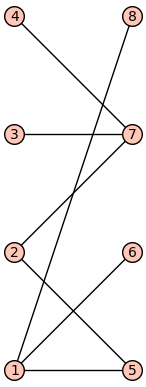
\includegraphics[width=0.15\textwidth]{Images/BipartiteMatchings/bipartite_graph.png}
 \end{outImage}
\begin{sageCell}
    G.bipartite_sets()
\end{sageCell}
\begin{outCell}
    ({1, 2, 3, 4}, {8, 5, 6, 7})
\end{outCell}
\begin{sageCell}
    max_bipartite_matching(G)
\end{sageCell}
\begin{outCell}
    [(1, 6), (2, 5), (3, 7)]
\end{outCell}
\begin{sageCell}
    G.show(edge_colors={"red": max_bipartite_matching(G)})
\end{sageCell}
\begin{outImage}
    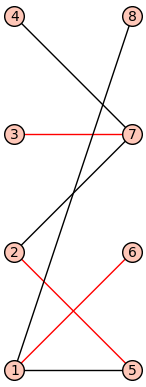
\includegraphics[width=0.15\textwidth]{Images/BipartiteMatchings/bipartite_graph_matching.png}
 \end{outImage}

 \subsubsection*{Minimum bipartite cover}

\begin{sageCell}
def min_bipartite_cover(G):
    A, B = G.bipartite_sets()
    Gp = DiGraph()
    Gp.add_vertices(G.vertices())
    s = Gp.add_vertex()
    t = Gp.add_vertex()
    Gp.add_edges([(s, a, 1) for a in A])
    Gp.add_edges([(b, t, 1) for b in B])
    for a in A:
        Gp.add_edges([(a, b, G.num_verts()) for b in G.neighbors(a)])
    _, _, sets = Gp.edge_cut(s, t, vertices=True)
    return [v for v in A if v in sets[1]] + [v for v in B if v in sets[0]]
\end{sageCell}
Example:
\begin{sageCell}
    G.show(vertex_colors={"red": min_bipartite_cover(G)})
\end{sageCell}
\begin{outImage}
    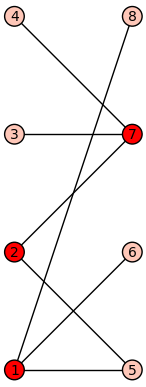
\includegraphics[width=0.15\textwidth]{Images/BipartiteMatchings/bipartite_graph_cover.png}
\end{outImage}


